\documentclass{article}
\usepackage{graphicx}
\usepackage{amsmath}
\usepackage{amsfonts}
\usepackage[parfill]{parskip}
\usepackage{hyperref}
\usepackage[useregional]{datetime2}
\usepackage[toc,page]{appendix}

\usepackage{biblatex}
\addbibresource{references.bib}

\usepackage[T1]{fontenc}
\usepackage{tgbonum}

\usepackage{listings}
\usepackage{xcolor}

\usepackage{longtable}

% Define a custom color
\definecolor{backcolour}{rgb}{0.95,0.95,0.92}
\definecolor{codegreen}{rgb}{0,0.6,0}

% Define a custom style
\lstdefinestyle{myStyle}{
    backgroundcolor=\color{backcolour},   
    commentstyle=\color{codegreen},
    basicstyle=\ttfamily\footnotesize,
    breakatwhitespace=false,         
    breaklines=true,                 
    keepspaces=true,                 
    numbers=left,       
    numbersep=5pt,                  
    showspaces=false,                
    showstringspaces=false,
    showtabs=false,                  
    tabsize=2,
}

% Use \lstset to make myStyle the global default
\lstset{style=myStyle}

\graphicspath{ {./figures/} }

\title{ELEC-E5510: Speech Recognition\\
    \large Project report: TITLE}

\newcommand{\inlinemaketitle}{{\let\newpage\relax\maketitle}}

\def\sectionautorefname{Section}

\begin{document}

\inlinemaketitle
\tableofcontents
% \newpage

% \listoffigures
% \newpage

% Content of report would be written here
% \include{./tex/task1.tex}
% ...
% \include{./tex/task2.tex}

\printbibliography[heading=bibintoc]

% \newpage
% \begin{appendices}
%     \section{Code}
All code is publicly accessible at \url{https://github.com/ancuongnguyen07/Multimodal-ERC/tree/master/code}

\begin{lstlisting}[label={lst:training-script},caption=Running the training script.]
python train_MELD.py --features-type text_audio_visual \
    --data-path data/MELD_features_raw1.pkl --output-dir models/
\end{lstlisting}

\begin{lstlisting}[label={lst:testing-script},caption=Running the testing script.]
python test_MELD.py --model-path ../models/text_audio_visual_BiDi_Att.pth \
    --features-type text_audio_visual
\end{lstlisting}

\section{Confusion Matrices}
\begin{figure}[htbp]
    \centering
    \begin{subfigure}[b]{0.45\textwidth}
        \centering
        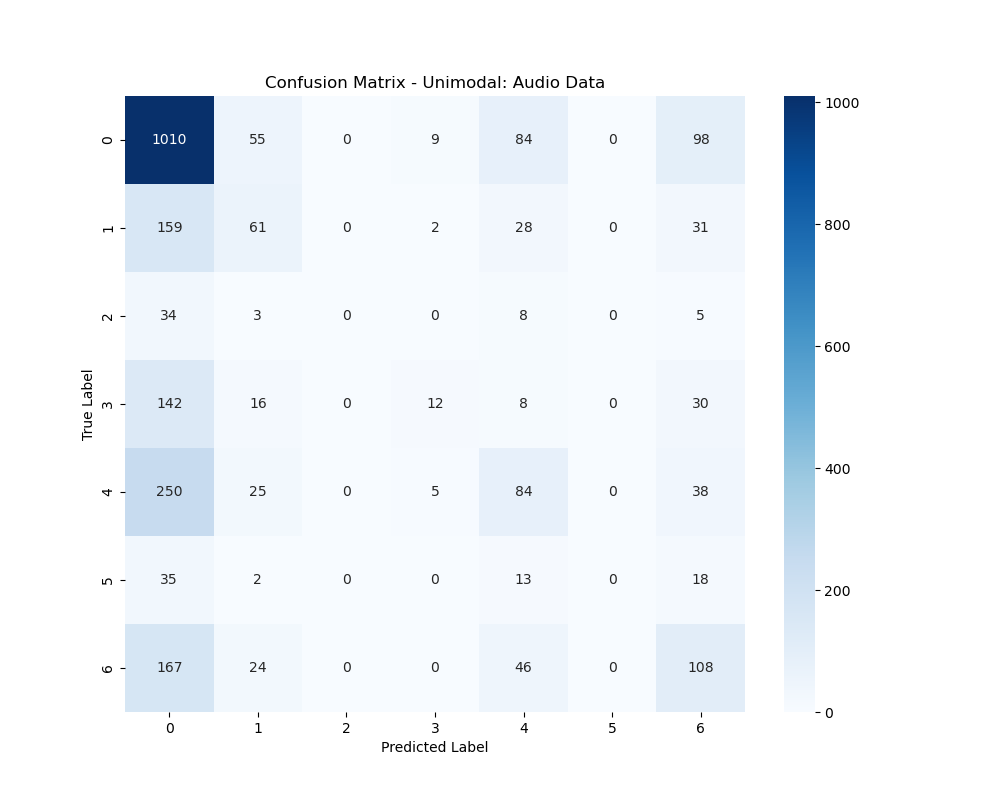
\includegraphics[width=\textwidth]{figures/audio.png}
        \caption{Unimodal: Audio Data}
    \end{subfigure}
    \hfill
    \begin{subfigure}[b]{0.45\textwidth}
        \centering
        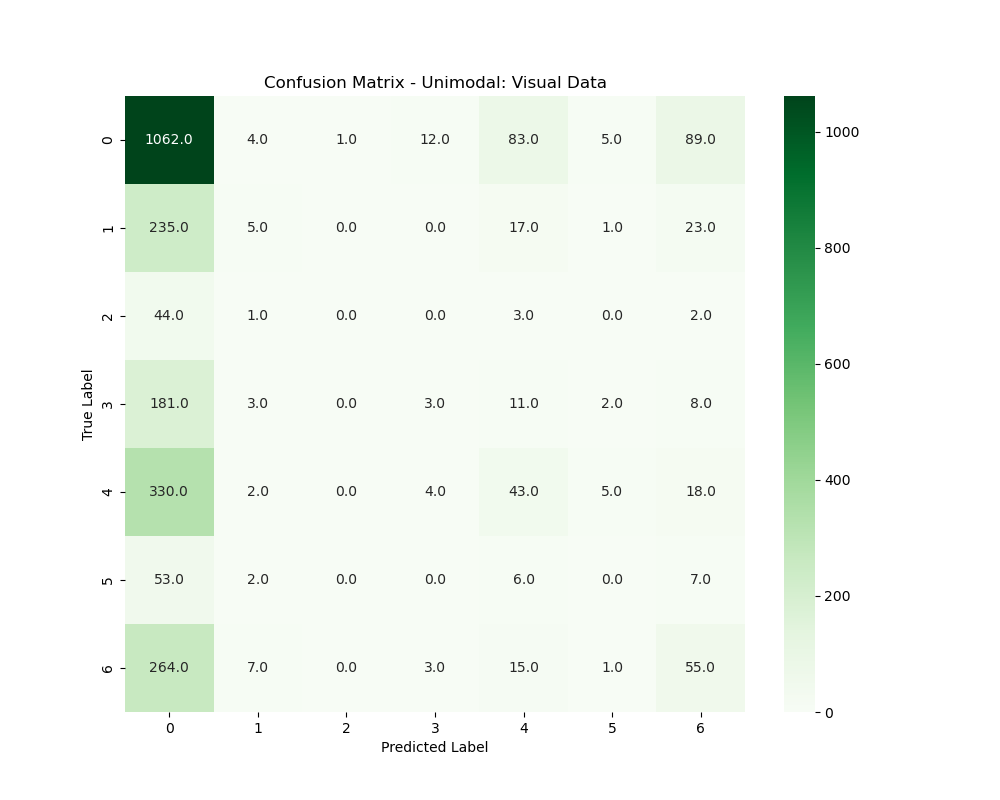
\includegraphics[width=\textwidth]{figures/visual.png}
        \caption{Unimodal: Visual Data}
    \end{subfigure}

    \vspace{0.5cm} % Vertical space between rows

    \begin{subfigure}[b]{0.45\textwidth}
        \centering
        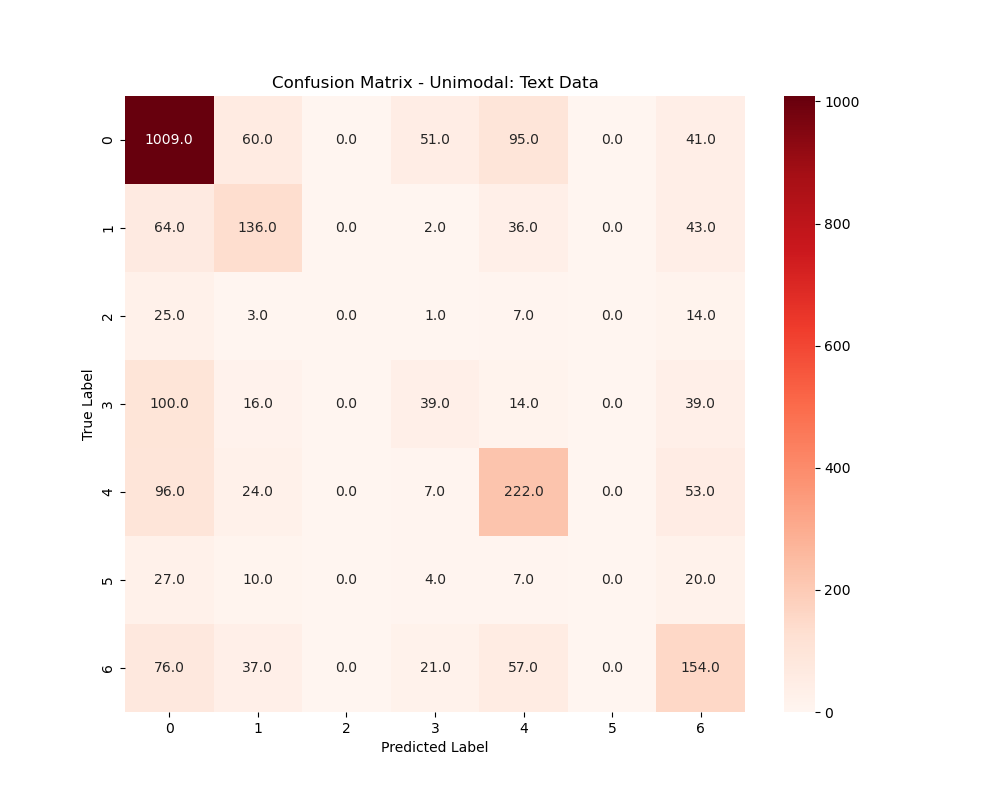
\includegraphics[width=\textwidth]{figures/text.png}
        \caption{Unimodal: Text Data}
    \end{subfigure}
    \hfill
    \begin{subfigure}[b]{0.45\textwidth}
        \centering
        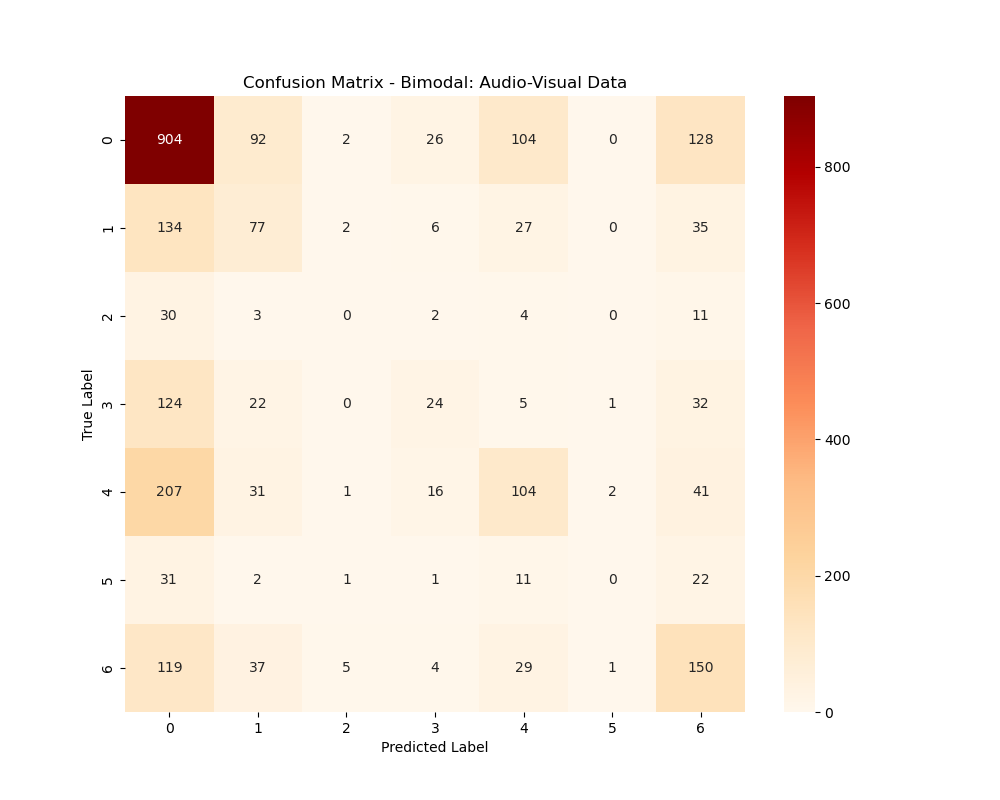
\includegraphics[width=\textwidth]{figures/audio-visual.png}
        \caption{Bimodal: Audio-Visual Data}
    \end{subfigure}

    \vspace{0.5cm} % Vertical space between rows

    \begin{subfigure}[b]{0.45\textwidth}
        \centering
        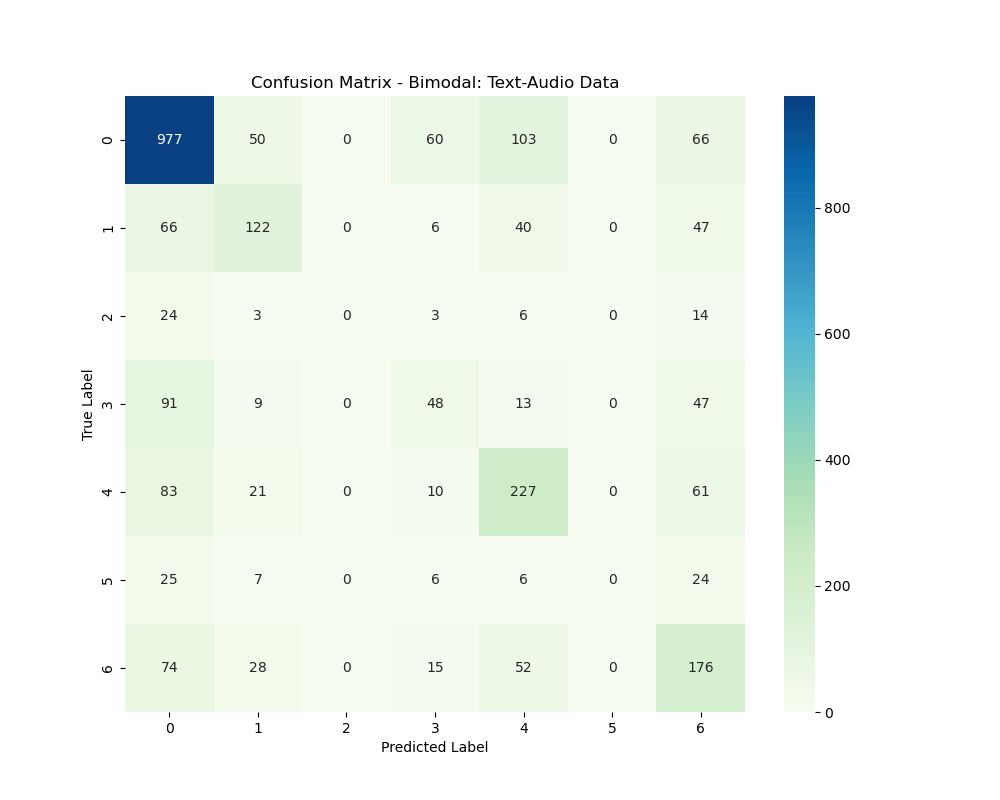
\includegraphics[width=\textwidth]{figures/text-audio.png}
        \caption{Bimodal: Text-Audio Data}
    \end{subfigure}
    \hfill
    \begin{subfigure}[b]{0.45\textwidth}
        \centering
        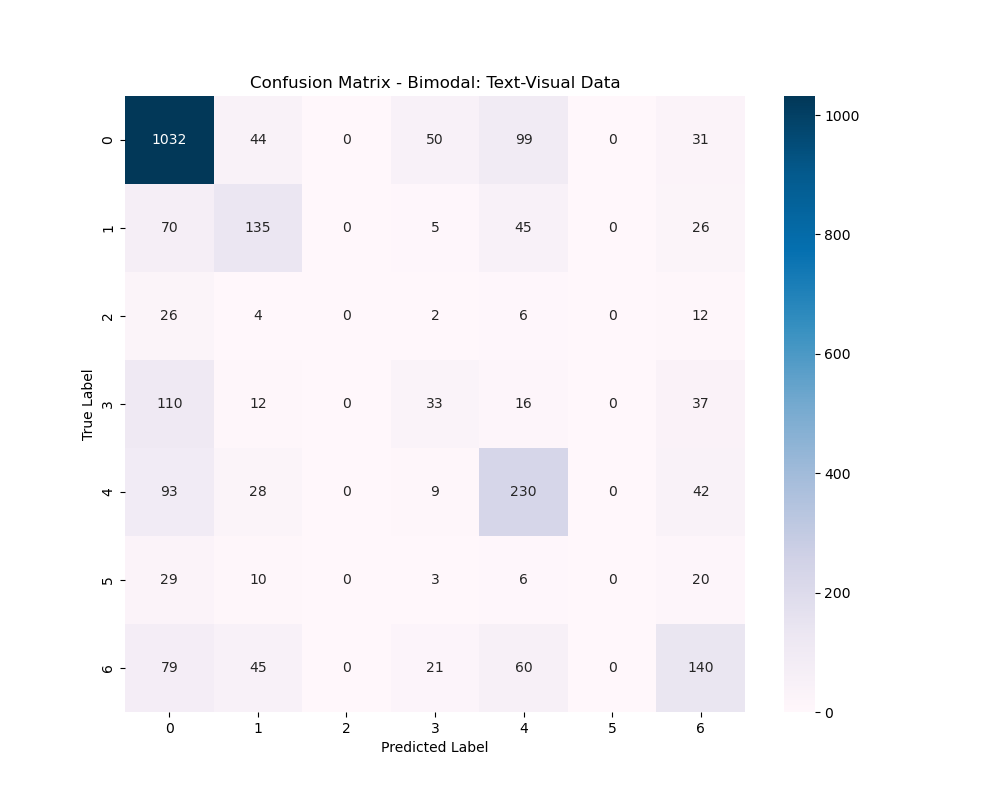
\includegraphics[width=\textwidth]{figures/text-visual.png}
        \caption{Bimodal: Text-Visual Data}
    \end{subfigure}

    \vspace{0.5cm} % Vertical space between rows

    \begin{subfigure}[b]{0.45\textwidth}
        \centering
        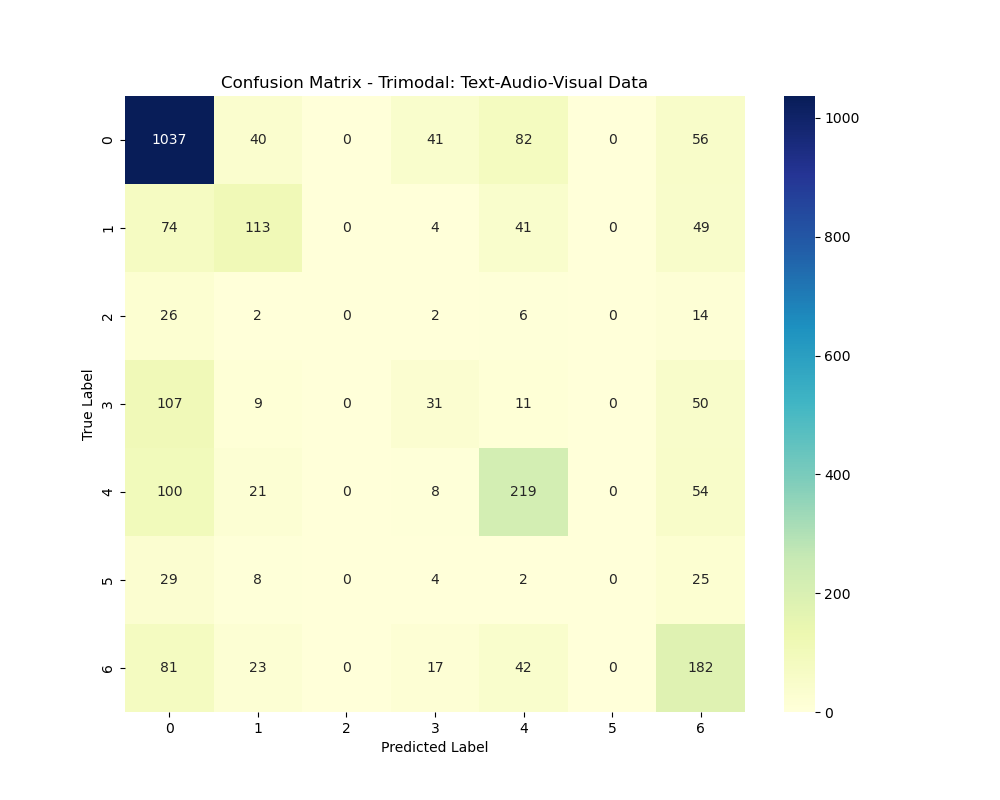
\includegraphics[width=\textwidth]{figures/text-audio-visual.png}
        \caption{Trimodal: Text-Audio-Visual Data}
    \end{subfigure}

    \caption{Confusion Matrices Across Modalities}
    \label{fig:confusion_matrices}
\end{figure}
% \end{appendices}

\end{document}
